\chapter{STARPY: A Bayesian analysis of a galaxy's SFH}

\emph{The work in the following chapter has been published in \citet{smethurst15}.}
\\

In order to achieve robust conclusions we conduct a Bayesian analysis \citep{Sivia, MacKay} of our SFH models in comparison to the observed GZ2 sample data. This approach requires consideration of all possible combinations of $\theta \equiv (t_{q}, \tau)$. Assuming that all galaxies formed at $t=0~\rm{Gyr}$ with an initial burst of star formation, we can assume that the `age' of each galaxy in the GZ2 sample is equivalent to an observed time, $t^{obs}_{k}$ (see Section~\ref{class}). We then use this  `age' to calculate the predicted model colours at this cosmic time for a given combination of $\theta$: $d_{c,p}(\theta_k, t^{obs}_{k})$ for both optical and NUV $(c={opt,NUV})$ colours. We can now directly compare our model colours with the observed GZ2 galaxy colours, so that for a single galaxy $k$ with optical ($u-r$) colour, $d_{opt, k}$ and NUV ($NUV-u$) colour, $d_{NUV,k}$, the likelihood $P(d_{k}|\theta_k, t^{obs}_{k})$ is:


\begin{equation}\label{like}
P(d_{k}|\theta_k, t^{obs}_{k}) = \frac{1}{\sqrt{2\pi\sigma_{opt, k}^2}}\frac{1}{\sqrt{2\pi\sigma_{NUV, k}^2}} \\ \exp{\left[ - \frac{(d_{opt, k} - d_{opt, p}(\theta_k, t_{k}^{obs}))^2}{\sigma_{opt, k}^2} \right]} \\ \exp{\left[ - \frac{(d_{NUV, k} - d_{NUV, p}(\theta_k, t_{k}^{obs}))^2}{\sigma_{NUV, k}^2} \right]}.
\end{equation}


We have assumed that $P(d_{opt}|\theta_k, t^{obs}_{k})$ and $P(d_{NUV}|\theta_k, t^{obs}_{k})$ are independent of each other and that the errors on the observed colours are also independent. To obtain the probability of each combination of $\theta$ values \underline{given} the GZ2 data: $P(\theta_k|d_k, t^{obs})$, i.e. how likely is a single SFH model given the observed colours of a single GZ2 galaxy, we utilise Bayes' theorem:
 \begin{equation}\label{big}
P(\theta_k|d_k, t^{obs}) = \frac{P(d_k|\theta_k, t^{obs})P(\theta_k)}{\int P(d_k |\theta_k, t^{obs})P(\theta_k) d\theta_k}.
\end{equation}
We assume a flat prior on the model parameters so that:
\begin{equation}\label{prior}
P(\theta_k) =
\begin{cases}
1 & \text{if } 0 \leq t_q ~\rm{[Gyr]}~ \leq 13.8 ~  \text{ and } ~ 0 \leq \tau  ~\rm{[Gyr]}~ \leq 4\\
0 & \text{otherwise.} \\
\end{cases}
\end{equation}

\begin{figure}
\centering{
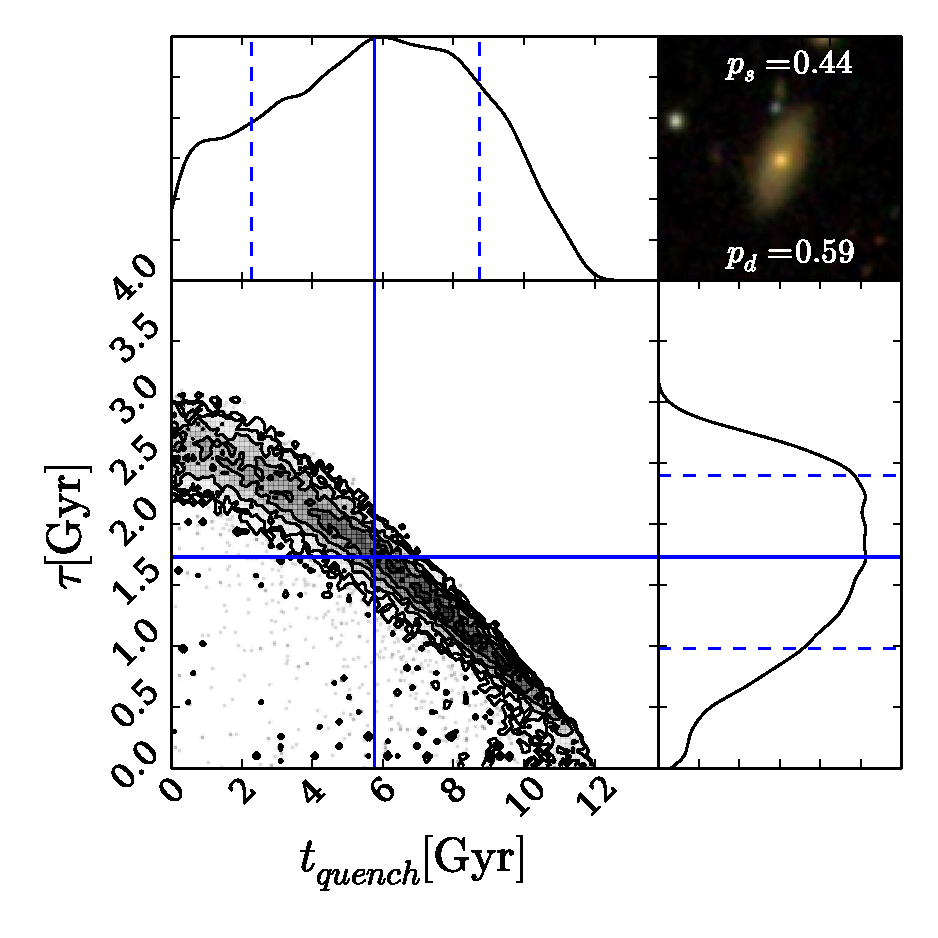
\includegraphics[width=0.9\textwidth]
{starpy/triangle_t_tau_red_s_1237655504035185152_40000_14_16_06_08_14.pdf}
\caption{Example output from \starpy ~for a galaxy within the red sequence. The contours show the positions of the `walkers' in the Markov Chain (which are analogous to the areas of high probability) for the quenching models described by $\theta = [t_q, \tau]$ and the histograms show the 1D projection along each axis. Solid (dashed) blue lines show the best fit model (with $\pm 1\sigma$) to the galaxy data. The postage stamp image from SDSS is shown in the top right along with the debiased vote fractions for smooth ($p_s$) and disc ($p_d$) from Galaxy Zoo 2.} }
\label{one_example}
\end{figure}

As the denominator of Equation~\ref{big} is a normalisation factor, comparison between likelihoods for two different SFH models (i.e., two different combinations of $\theta_k = [t_q, \tau]$) is equivalent to a comparison of the numerators. Calculation of $P(\theta_k|d_k, t^{obs})$  for any $\theta$ is possible given galaxy data from the GZ2 sample. Markov Chain Monte Carlo (MCMC; \citealt{MacKay, Dan, GW10}) provides a robust comparison of the likelihoods between $\theta$ values; here we choose \emph{emcee},\footnote{\url{dan.iel.fm/emcee/}} a Python implementation of an affine invariant ensemble sampler by \cite{Dan}.

This method allows for a more efficient exploration of the parameter space by avoiding those areas with low likelihood. A large number of `walkers' are started at an initial position where the likelihood is calculated; from there they individually `jump' to a new area of parameter space. If the likelihood in this new area is greater (less) than the original position then the `walkers' accept (reject) this change in position. Any new position then influences the direction of the  `jumps' of other walkers. This is repeated for the defined number of steps after an initial `burn-in' phase. \emph{emcee} returns the positions of these `walkers', which are analogous to the regions of high probability in the model parameter space. The model outlined above has been coded using the \emph{Python} programming language into a package named \starpy ~which has been made freely available to download\footnote{\url{github.com/zooniverse/starpy}}. An example output from this Python package for a single galaxy from the GZ2 sample in the red sequence is shown in Figure~\ref{one_example}. The contours show the positions of the `walkers' in the Markov Chain which are analogous to the areas of high probability.

\begin{figure}
\centering{
\includegraphics[width=\textwidth]{starpy/mosaic_test.pdf}}
\caption{Results from \starpy ~for an array of synthesised galaxies with known, i.e. \underline{true}, $t_q$ and $\tau$ values (marked by the red lines) using the complete function to calculate the predicted colour of a proposed set of $\theta$ values in each MCMC iteration, assuming an error on the calculated known colours of $\sigma_{u-r} = 0.124$ and $\sigma_{NUV-u} = 0.215$, the average errors on the GZ sample colours. In each case \starpy ~succeeds in locating the true parameter values within the degeneracies of the star formation history model. These degeneracies can clearly be seen in Figure~\ref{pred}.}
\label{test_mosaic}
\end{figure}

In order to test that \starpy ~can find the correct quenching model for a given observed colour, 25 synthesised galaxies were created with known SFHs (i.e. known values of $\theta$) from which optical and NUV colours were generated. These were input into \starpy ~ to ensure that the known values of $\theta$ were reproduced, within error, for each of the 25 synthesised galaxies. Figure~\ref{test_mosaic} shows the results for each of these 25 synthesised galaxies, with the known values of $\theta$ shown by the red lines. In some cases this red line does not coincide with the peak of the distribution shown in the histograms for one parameter, however in all cases the intersection of the red lines is within the sample contours. 

We find peaks in the histograms across all areas of the parameter space in both dimensions of $[t, \tau]$, this ensures that the results presented in Figures~\ref{red_s},~\ref{green_v} \&~\ref{blue_c} arise due to a superposition of extended probability distributions, as opposed to a bimodal distribution of probability distributions across all galaxies.


\begin{figure*}
\centering{
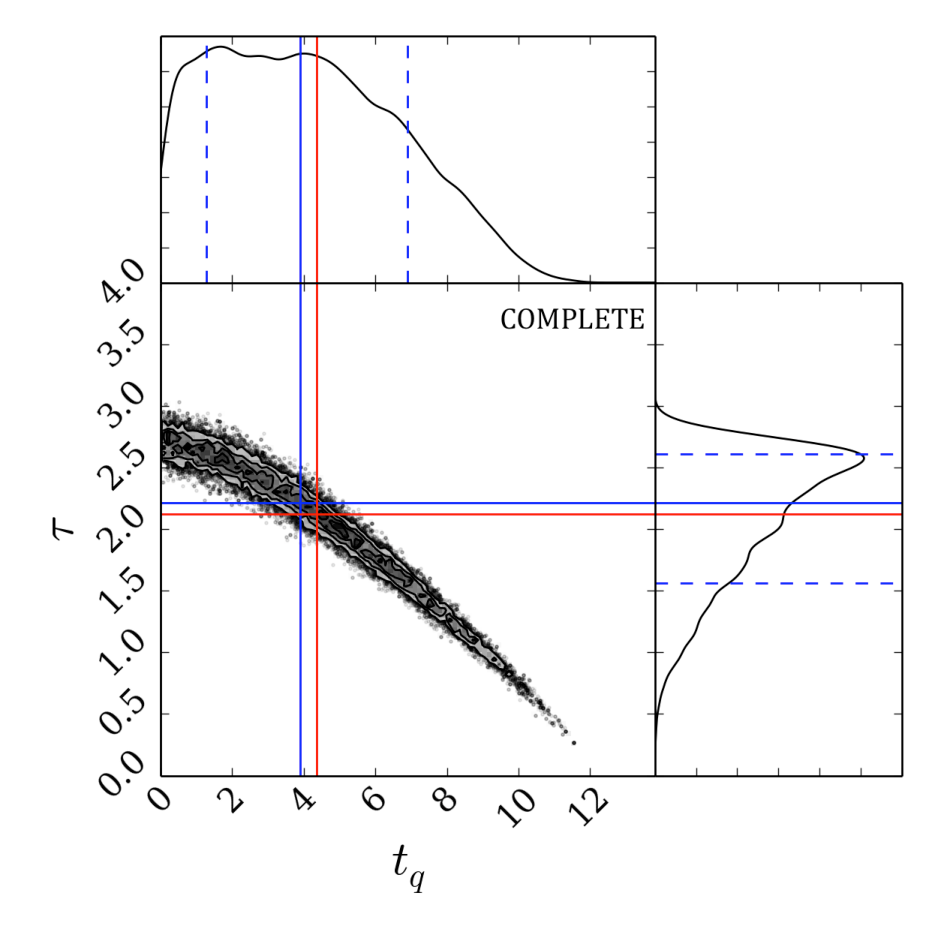
\includegraphics[width=0.49\textwidth]{starpy/corner_test_starfpy_full_sfh_function_0.pdf}
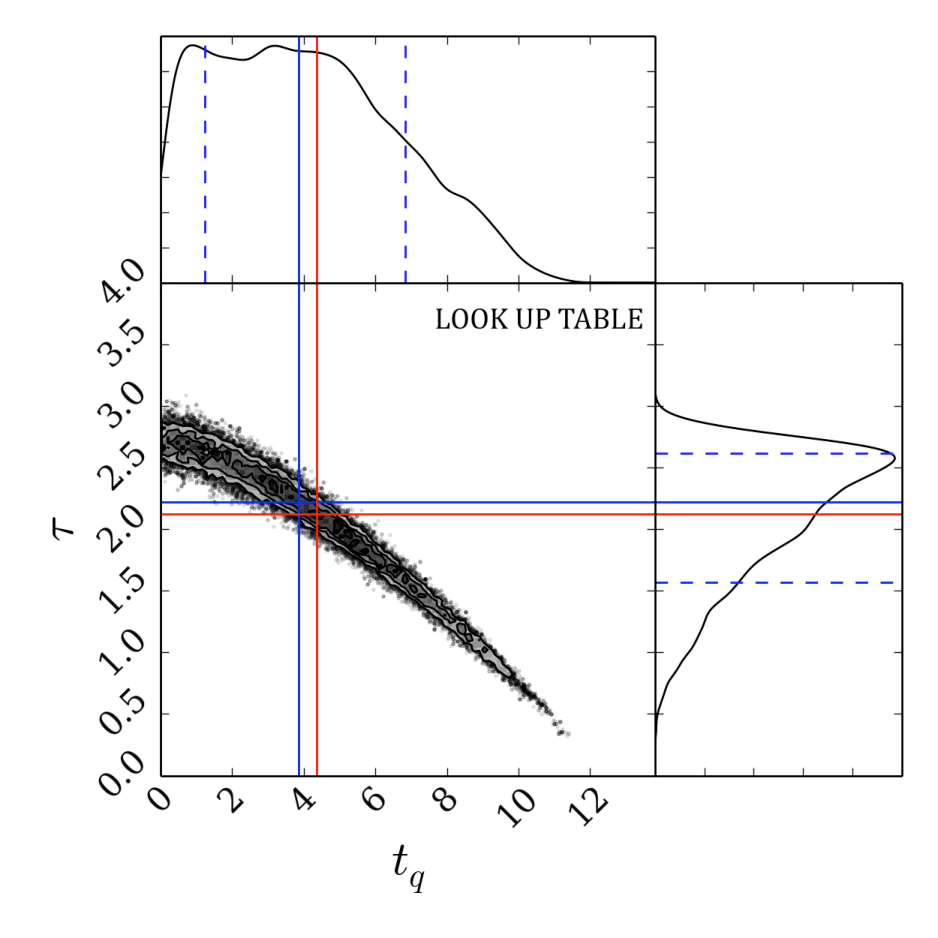
\includegraphics[width=0.49\textwidth]{starpy/corner_test_starfpy_lookup_0.pdf}}
\caption{Left panel: Results from \starpy ~for \underline{true} $t_q$ and $\tau$ values (red lines) using the complete function to calculate the predicted colour of a proposed set of $\theta$ values in each MCMC iteration. The median walker position (the 50th percentile of the Bayesian probability distribution) is shown by the solid blue line with the dashed lines encompassing $68\% (\pm 1\sigma)$ of the samples (the 16th and 84th percentile positions). The time taken to run for a single galaxy using this method is approximately 2 hours. Right panel: Results from \starpy ~for \underline{true} $t_q$ and $\tau$ values using a look up table generated from the complete function to calculate the predicted colour of a proposed set of $\theta$ values in each MCMC iteration. The time taken to run for a single galaxy using this method is approximately 2 minutes.}
\label{lookup}
\end{figure*}

\begin{table}
\centering{
\caption{Median walker positions (the 50th percentile; as shown by the blue solid lines in Figure~\ref{lookup}) found by \starpy ~ for a single galaxy, using the complete star formation history function and a look up table to speed up the run time. The errors quoted define the region in which $68\%$ of the samples are located, shown by the dashed blue lines in Figure~\ref{lookup}. The known true values are also quoted, as shown by the red lines in Figure~\ref{lookup}. All values are quoted to three significant figures.}
\begin{tabular*}{0.65\textwidth}{r @{\extracolsep{\fill}}ccc}
\multicolumn{1}{l}{} & \multicolumn{3}{c}{}                                          \\ \hline
                     & $t_q$                       & $\tau$                       &  \\ \hline
True                 & $4.37$                        & $2.12$                         &  \\
Complete             & $3.893 \pm^{3.014}_{2.622}$ & $2.215 \pm^{0.395}_{0.652}$ &  \\
Look up table        & $3.850 \pm^{2.988}_{2.619}$ & $2.218 \pm^{0.399}_{0.649}$ & \\ \hline
\end{tabular*}}
\label{median_lu}
\end{table}

Considering the size of the sample in this investigation of $126,316$ galaxies total, a three dimensional look up table (in observed time, quenching time and quenching rate) was generated using the star formation history function in \starpy ~to speed up the run time. 

We wish to consider the model parameters for the populations of galaxies across the colour magnitude diagram for both smooth and disc galaxies, therefore we run the \starpy ~package on each galaxy in the GZ2 sample. This was extremely time consuming; for each combination of $\theta$ values which \emph{emcee} proposes, a new SFH must be built, prior to convolving it with the BC03 SPS models at the observed age and then predicted colours calculated from the resultant SED. For a single galaxy this takes up to 2 hours on a typical desktop machine for long Markov Chains. A look-up table was therefore generated at $50 ~t^{obs}$, for $100 ~t_{quench}$ and $100 ~\tau$ values; this was then interpolated over for a given observed galaxy's age and proposed $\theta$ values at each step in the Markov Chain. This ensures that a single galaxy takes approximately 2 minutes to run on a typical desktop machine. Figure~\ref{lookup} shows an example of how using the look up table in place of the full function does not affect the results to a significant level. Table~\ref{median_lu} quotes the median walker positions (the 50th percentile of the Bayesian probability distribution) along with their $\pm 1\sigma$ ranges for both methods in comparison to the true values specified to test \starpy. The uncertainties incorporated into the quoted values by using the look up table are therefore minimal with a maximum $\Delta = 0.043$.

Using this lookup table, each of the $126,316$ total galaxies in the GZ2 sample was run through \starpy ~on multiple cores of a computer cluster to obtain the Markov Chain positions (analogous to $P(\theta_k|d_k)$) for each galaxy, $k$ (see Figure~\ref{one_example}). In each case the Markov Chain consisted of $100$ `walkers' which took $400$ steps in the `burn-in' phase and $400$ steps thereafter, at which point the MCMC acceptance fraction was checked to be within the range $0.25 < f_{acc} < 0.5$ (which was true in all cases). Due to the Bayesian nature of this method, a statistical test on the results is not possible; the output is probabilistic in nature across the entirety of the parameter space.

These individual galaxy positions are then combined to visualise the areas of high probability in the model parameter space across a given population (e.g. the green valley). 

\begin{table*}
\centering{
\caption{Number of galaxies in each population which had walker positions discarded due to low probability in order to exclude those galaxies from the analysis which were poorly fit by this quenching model.}
\begin{tabular*}{0.95\textwidth}{p{4cm} @{\extracolsep{\fill}} ccc}
                                          & \textbf{Red Sequence}                                   & \textbf{Green Valley}                                  & \textbf{Blue Cloud}                                      \\ \hline
All walkers discarded                     & \begin{tabular}[c]{@{}c@{}}1420\\ (7.00\%)\end{tabular} & \begin{tabular}[c]{@{}c@{}}437\\ (2.41\%)\end{tabular} & \begin{tabular}[c]{@{}c@{}}3109\\ (5.37\%)\end{tabular}  \\
More than half walker positions discarded & \begin{tabular}[c]{@{}c@{}}2010\\ (9.92\%)\end{tabular} & \begin{tabular}[c]{@{}c@{}}779\\ (4.30\%)\end{tabular} & \begin{tabular}[c]{@{}c@{}}6669\\ (11.52\%)\end{tabular} \\ \hline
\end{tabular*}}
\label{discardnum}
\end{table*}

We discard walker positions returned by \starpy~ with a corresponding probability of $P(\theta_k|d_k) < 0.2$ in order to exclude galaxies which are not well fit by the quenching model; for example blue cloud galaxies which are still star forming will be poorly fit by a quenching model (see Section~\ref{qmod}). This raises the issue of whether we exclude a significant fraction of our galaxy sample and whether those galaxies reside in a specific location of the colour-magnitude. The fraction of galaxies which had all or more than half of their walker positions discarded due to low probability are shown in Table \ref{discardnum}. Using this constraint, $2.4\%$, $7.0\%$ and $5.4\%$ of green, red and blue galaxies respectively had \emph{all} of their walker positions discarded. 

This is not a significant fraction of either population, therefore this shows that the \starpy~ module is effective in fitting the majority of galaxies and that this method of discarding walker positions ensures that poorly fit galaxies are removed from the analysis of the results. Figure \ref{discarded} shows that these galaxies with discarded walker positions are also scattered across the optical-NUV colour-colour diagram and therefore \starpy ~is also effective in fitting galaxies across this entire plane. 

\begin{figure}
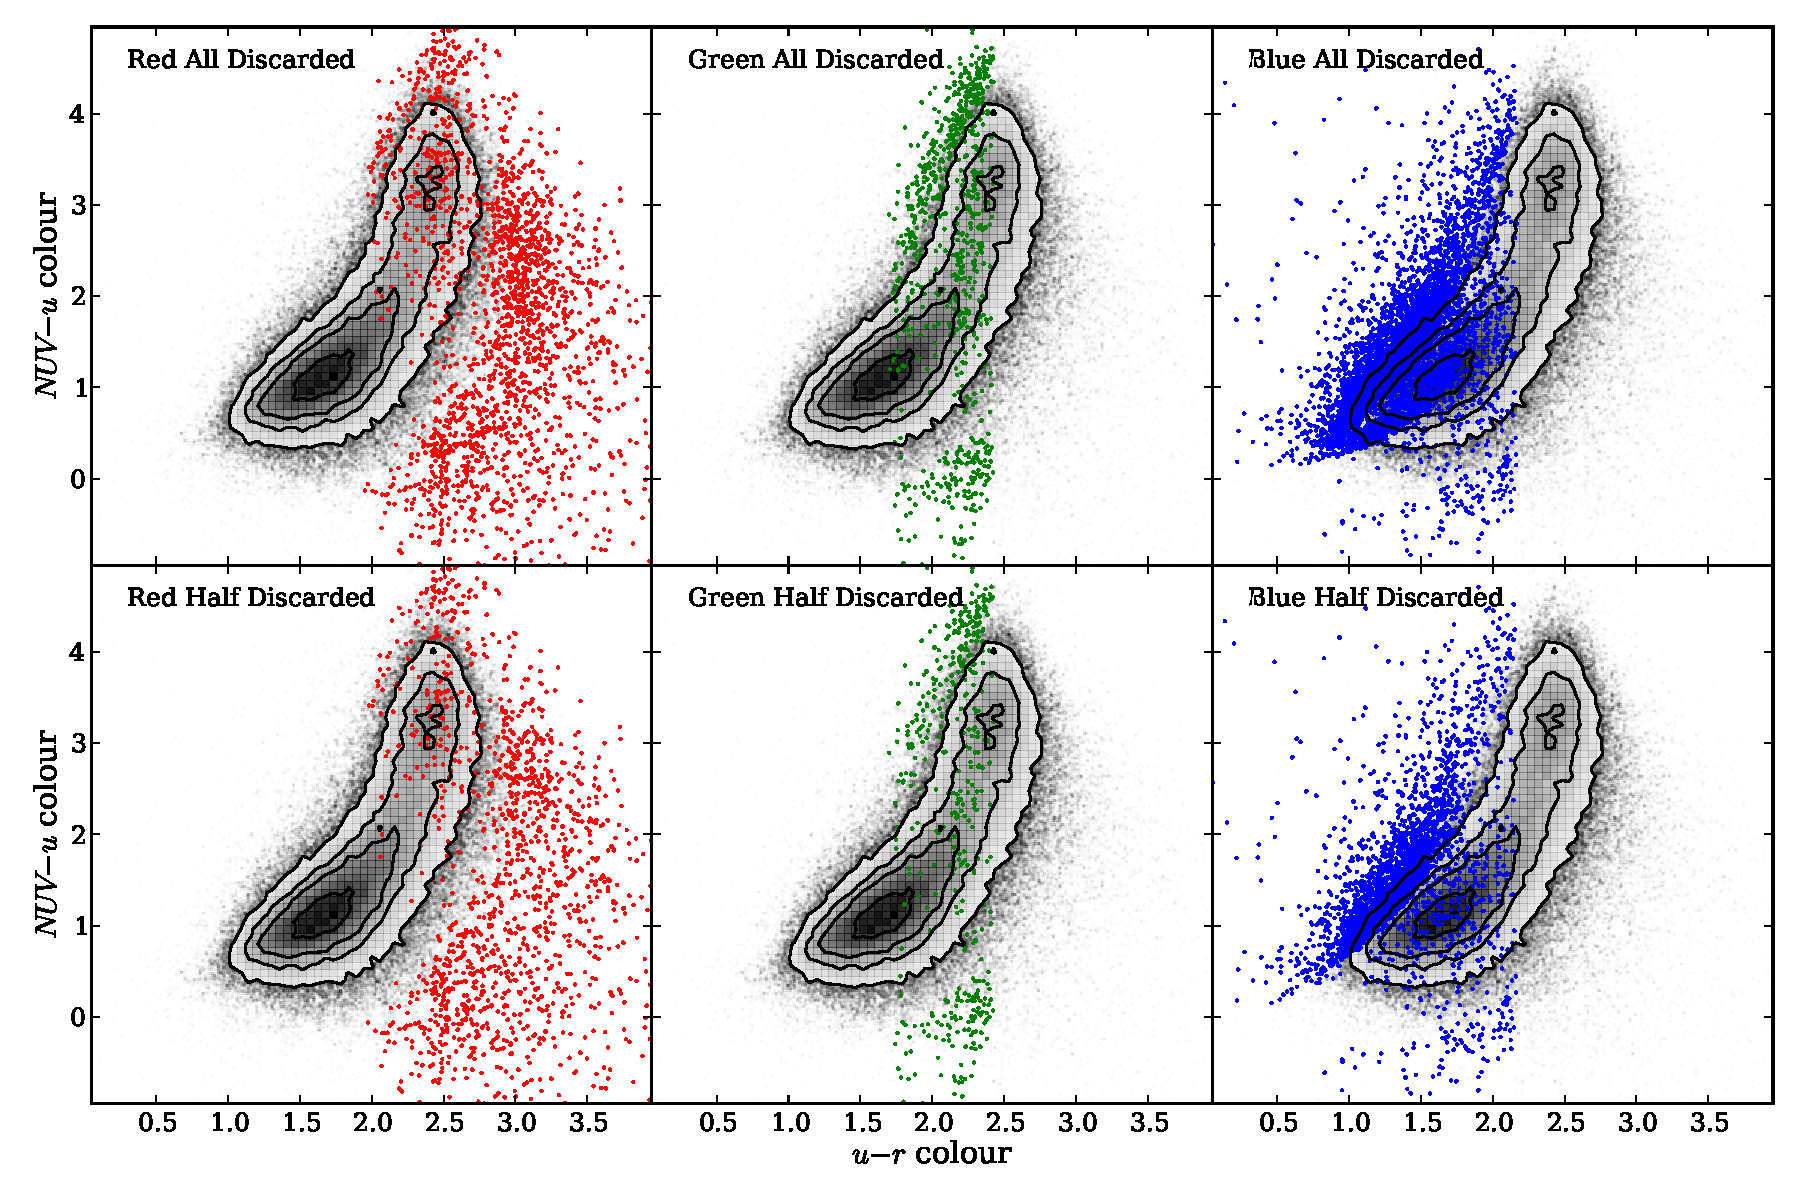
\includegraphics[width=0.9\textwidth]{starpy/discarded_galaxy_colour_colour.pdf}
\caption{Contours show the full GZ2 subsample optical-NUV colour-colour diagram. The points show the positions of the galaxies which had all (top panels) or more than half (bottom panel) of their walker positions discarded due to their low probability for the red sequence (left), green valley (middle) and blue cloud (right).}
\label{discarded}
\end{figure}



The Markov Chain positions are then binned and weighted by their corresponding logarithmic posterior probability $\log [P(\theta_k|d_k)]$, provided by the \emph{emcee} package, to further emphasise the features and differences between each population in the visualisation. The GZ2 data also provides uniquely powerful continuous measurements of a galaxy's morphology, therefore we utilise the user vote fractions to obtain separate model parameter distributions for both smooth and disc galaxies. This is obtained by also weighting by the morphology vote fraction when the binned positions are summed. We stress that this portion of the methodology is a non-Bayesian visualisation of the combined individual galaxy results for each population.

For example, the galaxy shown in Figure~\ref{one_example} would contribute almost evenly to both the smooth and disc parameters due to the GZ2 vote fractions. Since galaxies with similar vote fractions contain both a bulge and disc component, this method is effective in incorporating intermediate galaxies which are thought to be crucial to the morphological changes between early- and late-type galaxies. It was the consideration of these intermediate galaxies which was excluded from the investigation by S14.
